Earlier in \ref{Existing} page \pageref{Existing} we looked at a broad spectrum of recommendation techniques and  split them into three groups and a fourth being a combination of the first three. Now we will look closer at what we earlier identified as the personal and social recommendations, when looking at them from a more technical standpoint it makes more sense to group them after what sources they use and how they use them.

\begin{figure}[H]
\centering
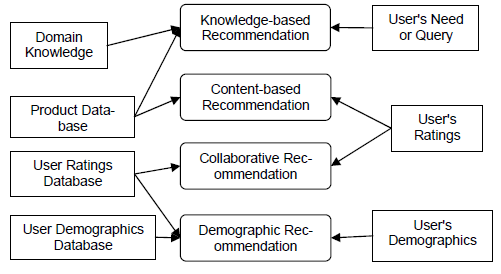
\includegraphics[width=0.8\textwidth]{Images/RecTypes.png}
\caption{Recommendation Techniques and their knowledge sources. Picture from \cite{TheAdaptiveWeb}}
\label{RecTypes}
\end{figure}

Picture \ref{RecTypes} shows the four recommendation systems and what sources they use. Sometimes the sources available dictates which recommender the system must use unless a hybrid is chosen. 


\subsubsection{Collaborative Recommendations} 
\label{Collaborative} 
\relinput{Collaborative} 

\subsubsection{Content Based Recommendations} 
\label{ContentBased} 
\relinput{ContentBased}

\subsubsection{Differences}
\label{Differences} 
\relinput{Differences}

\subsubsection{Hybrid Systems} 
\label{Hybrid} 
\relinput{Hybrid}